%!TeX root=main.tex
\chapter{مروری بر کار‌های مرتبط}
\thispagestyle{empty}

در حال حاضر تمرکز اصلی پژوهش‌های انجام شده در حوزه متن و تصویر دست‌یابی به دقت بالا با استفاده از شبکه‌های بزرگ ترنسفورمر می‌باشد. مدل‌های یادشده علاوه بر دقت بالا در مسائل، پیچیدگی محاسباتی و تعداد پارامتر‌های زیادی دارند. همین عامل موجب می‌شود استفاده از این مدل‌ها در کاربرد‌های زندگی حقیقی با مشکلاتی روبرو شود؛ زیرا به دستگاه‌هایی با پردازنده قوی و حافظه بالا نیاز دارند. بنابراین استفاده از مدل‌ها بر روی دستگاه‌های تلفن همراه که اغلب محدودیت پردازش و حافظه دارند، با چالش‌هایی روبرو شده است. 
\newline
از این رو امروزه پژوهش‌هایی در زمینه کاهش پارامتر‌های مدل و کاهش پیچیدگی محاسباتی انجام شده است. هدف این پژوهش‌ها کاهش پیچیدگی محاسباتی و کاهش تعداد پارامتر‌ها می‌باشد به طوری که دقت مدل دست خوش تغییر نشود. پژوهش‌ها را در دو دسته کلی زیر می‌توان طبقه‌بندی کرد. 
\begin{enumerate}
	\item معرفی معماری و ساختار جدید برای شبکه.
	\item فشرده‌سازی شبکه‌های از قبل معرفی شده با روش‌‌های مختلف.
\end{enumerate}
در ادامه به بررسی پژوهش‌های صورت گرفته در این حوزه پرداخته می‌شود.
\section{شبکه
	\lr{MiniVLM}}

شبکه
\lr{MiniVLM}
\LTRfootnote{\lr{Mini Vision-Language Model}}
یک مدل کوچک‌تر و سریع‌تر برای مسئله‌های تصویری-زبانی می‌باشد. با توجه به ویژگی یاد شده، این شبکه مناسب استفاده در دستگاه‌هایی با محدودیت حافظه و قدرت پردارش است. ساختار 
\lr{MiniVLM}
با هدف کاهش محاسبات ناشی از ساختار ترنسفورمر‌ها طراحی شده است. در پژوهش‌های انجام شده برای طراحی مدل
 \lr{MiniVLM}
 ابتدا معماری مدل برای دستیابی به سرعت و دقت مناسب، بهبود یافته و سپس بخش آموزش اولیه
 \LTRfootnote{\lr{pre-traning} }
  ارتقا داده شده است \cite{wang2020minivlm}.
\newline
 برای بخش تصویر از
\lr{Two-stage Efficient feature Extractor (TEE)}
استفاده شده است. استفاده از این ماژول هزینه استخراج ویژگی‌‌های تصویر را به میزان 
\lr{95}
درصد در مقایسه با شبکه
\lr{OSCAR}
\cite{li2020oscar}
\LTRfootnote{\lr{State Of The Art}}
کاهش داده است. در \lr{Two-stage Efficient feature Extractor (TEE)} به جای استفاده از لایه‌های پیچشی
\LTRfootnote{\lr{Convolution}}
 معمولی از لایه پیچشی نقطه‌ای
\LTRfootnote{\lr{Pointwise}}
و لایه پیچشی عمقی
\LTRfootnote{\lr{Depthwise}}
استفاده شده است.
\newline
برای ارتقا بخش آموزش اولیه و جبران کاهش تعداد پارامتر‌ها در شبکه \lr{MiniVLM}،
از مجموعه‌های بسیار بزرگ استفاده شده است.
\newline
در نتیجه همه تلاش‌ها زمان ابتدا به انتها این مدل در مقایسه با شبکه \lr{OSCAR} میزان 
\lr{6\%}
کاهش پیدا کرده است. تعداد پارامتر‌های شبکه \lr{MiniVLM}
\lr{27\% }
 پارامتر‌های \lr{OSCAR} می‌باشد. همچنین شبکه \lr{MiniVLM}، به
\lr{94\%-97\%}
  دقت شبکه \lr{OSCAR} دست یافته است. موارد مطرح شده نشان می‌دهد با وجود کاهش قابل توجه در تعداد پارامتر‌ها و همچنین افرایش سرعت مدل، دقت تغییر چندانی نکرده است. نتایج مقایسه دو شبکه در شکل
\ref{minivlm}
قابل مشاهده است.
\begin{figure}[H]
	\center{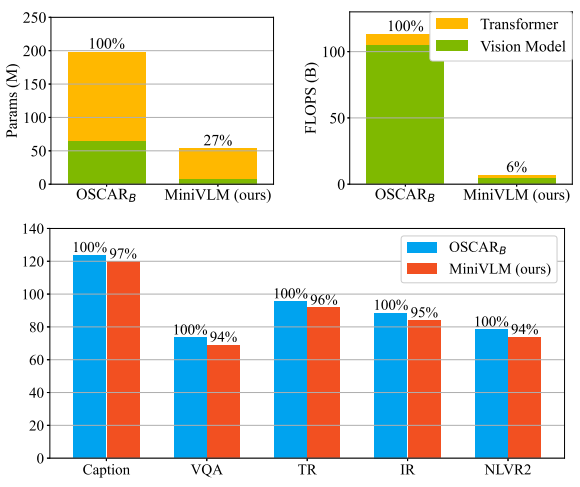
\includegraphics[width=0.7\linewidth]{images/minivlm.PNG}}
	\caption{مقایسه شبکه
		\lr{MiniVLM} و شبکه \lr{OSCAR}
		\cite{wang2020minivlm}}
	\label{minivlm}
\end{figure}

\iffalse	
\section{شبکه
	\lr{DistillVlM}}

تکمیل شود.
\fi
\section{فرضیه بلیط بخت‌آزمایی 
	%(\lr{Lottory Thicket Hypothesis})
} 
%\LTRfootnote{\lr{Lottory Thicket Hypothesis}}
در یادگیری ماشین تکنیک هرس 
\LTRfootnote{\lr{Pruning}}
شبکه عصبی، پارامتر‌های غیر ضروری شبکه را حذف می‌کند. با این روش می‌توان بدون کاهش چشم‌گیر در دقت شبکه، پارامتر‌های شبکه را به میزان قابل قبولی کاهش داد.  همچنین سرعت شبکه نسبت به حالت قبل هرس، افزایش پیدا می‌کند.
هدف اصلی در پژوهش یافتن بازنمایی کم‌حجم‌تر برای شبکه‌های عصبی کاملا متصل
\LTRfootnote{\lr{Dense Neural Network}}
می‌باشد تا موجب کاهش پیچیدگی محاسباتی شود. در مقاله فرضیه زیر اثبات شده است :
یک شبکه کاملا متصل که به صورت تصادفی مقدار دهی اولیه شده است
شامل یک زیر شبکه
\LTRfootnote{\lr{Subnetwork}}
می‌باشد به طوری که اگر آن زیر شبکه را به تعداد تکرار
\LTRfootnote{\lr{Iteration}}
مشابه شبکه اصلی آموزش دهیم، دقت روی داده تست در هر دو حالت یکسان خواهد شد \cite{frankle2019lottery}.
\newline \newline
نویسندگان مقاله فرضیه را بلیط بخت‌آزمایی
\LTRfootnote{\lr{Lottery Thicket Hypothesis}}
نام‌گذاری کردند و برای اثبات فرضیه علاوه بر شبکه عصبی متراکم
\LTRfootnote{\lr{Dence Neural Network}}
،
صحت فرضیه مطرح شده را بر روی شبکه پیچشی
\LTRfootnote{\lr{Convolutional Neural Network}}
بررسی کردند. در این مقاله الگوریتمی ارائه شده است که می‌تواند بلیط برنده 
\LTRfootnote{\lr{Winning Ticket}}
را پیدا کند. برای یافتن بلیط برنده در یک فرایند تکرار شونده
\LTRfootnote{\lr{Iterative}}
، اتصالات کم‌وزن شبکه را حذف می‌کنیم. سپس زیر شبکه جدید را دوباره آموزش می‌دهیم. این روش شبکه را کوچک‌‌تر می‌کند در حالی که دقت با حالت شبکه کامل تفاوتی ندارد. فرایند انجام آزمایش‌ها در این مقاله با هرس تکرارشونده
\LTRfootnote{\lr{Iterative Pruning}}
صورت گرفته است.


\subsection{هرس بر پایه وزن اتصالات}
در هرس بر پایه وزن اتصالات
\LTRfootnote{\lr{Magnitude Pruning}}
هدف این است که اتصالات شبکه با وزن کم نسبت به سایر اتصالات از شبکه حذف شود. ایده روش مطرح شده این است که اتصالات کم وزن، تاثیر کمتری در نتایج به دست آمده دارد. بنابراین حذف این اتصالات تغییر ناچیزی در عملکرد مدل دارد. پس می‌توان این اتصالات را حذف کرد.

\section{فرضیه بلیط بخت‌آزمایی در 
	\lr{UNITER}}
شبکه
\lr{UNITER}
\LTRfootnote{\lr{UNiversal Image-TExt Representation Learning}}\cite{chen2020uniter}
یکی از شبکه‌های معرفی شده در مسئله پرسش و پاسخ تصویری می‌باشد که به نتایج بسیار قابل قبولی دست یافته است. در راستا فشرده‌سازی شبکه‌های حجیم ترنسفورمری، پژوهشی به بررسی فشرده‌سازی و کاهش تعداد پارامتر‌های شبکه
\lr{UNITER}
پرداخته است. نتایج به دست آمده از این پژوهش نشان می‌دهد برای مسئله پرسش و پاسخ تصویری اگر 70 درصد اتصالات کم‌وزن شبکه کامل 
\lr{UNITER}
را هرس کنیم، دقت زیر‌شبکه جدید 99 درصد دقت شبکه کامل می‌باشد \cite{gan2021playing}.

%	\lr{playing lottory thicket with vision and language}